%! Author = Philipp Emmenegger
%! Date = 30/06/2021

\section{Protocols}
\subsection{Networking Layers}
\textbf{Goal:} Interoperability\\
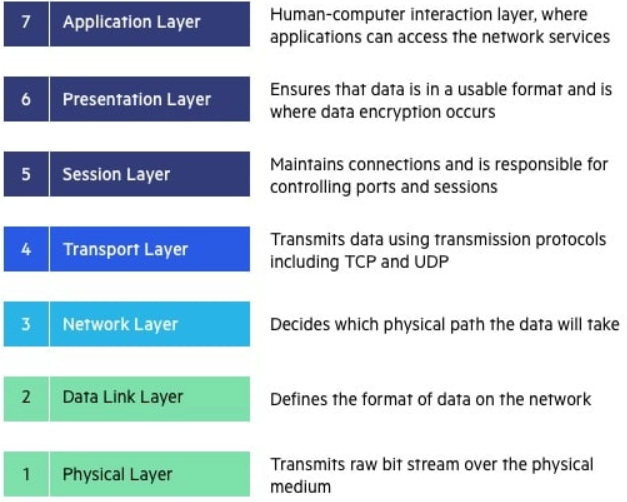
\includegraphics[width=0.6\linewidth]{img/osi_model.png}

\subsubsection{Layer Abstraction}
\begin{itemize}
    \item Protocols enable an entity to interact with an entity at the same layer in another host
    \item \textbf{Service definitions:} provide functionality to an (N)-layer by an (N-1) layer
    \item Layer N exchange protocol data units (PDUs) with layer N protocol
    \item Each PDU contains a header and payload, the service data unit (SDU)
\end{itemize}
\textbf{Example PDU of L3:}\\
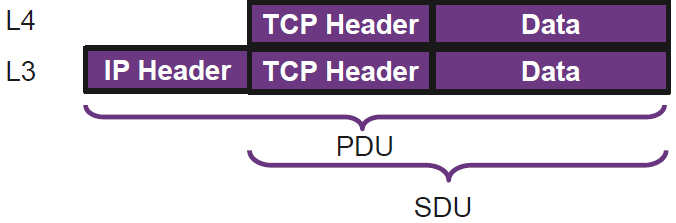
\includegraphics[width=0.6\linewidth]{img/pdu.png}

\subsection{Layer 4 - Transport}
\subsubsection{TCP}
\begin{itemize}
    \item Reliable
    \item Ordered
    \item Window - capacity of receiver
    \item Checksum - 16bit
    \item TCP overhead: 20 bytes
    \item Tries to correct errors
\end{itemize}
\textbf{Connection establishment}
\begin{itemize}
    \item SYN, SYN-ACK, ACK
    \item Initiates TCP session: initial sequence number is random
\end{itemize}
\textbf{Connection termination}
\begin{itemize}
    \item FIN, ACK + FIN, ACK
    \item 3-way handshake
\end{itemize}
\textbf{Sequences and ACKs}
\begin{itemize}
    \item Identification each byte of data
    \item Order of the bytes: reconstruction
    \item Detecting lost data: RTO, DupACK
\end{itemize}
\textbf{Retransmission timeout}
\begin{itemize}
    \item If no ACK is received after timeout
\end{itemize}
\textbf{Flow control}
\begin{itemize}
    \item Sender is not overwhelming a receiver
    \item Back pressure
    \item Sliding window
    \item Congestion control
    \begin{itemize}
        \item Slow-start
        \item Congestion avoidance
    \end{itemize}
\end{itemize}

\subsubsection{TCP + TLS}
\textbf{TLS \textless 1.3}
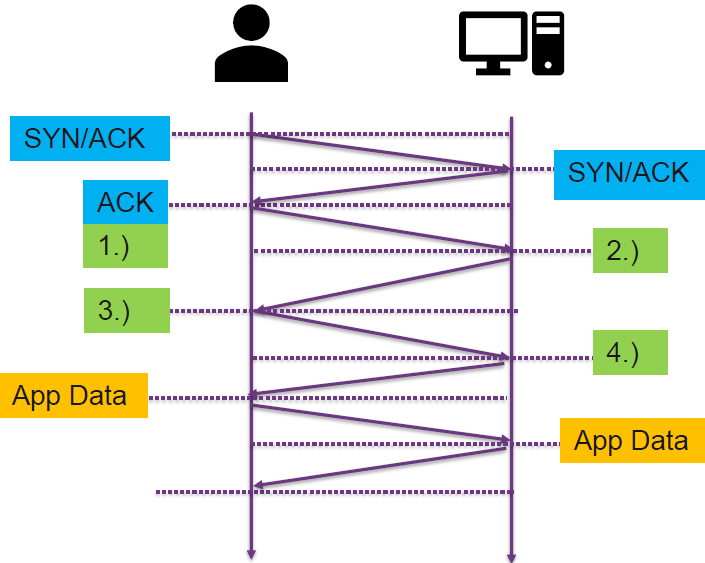
\includegraphics[width=0.7\linewidth]{img/tcp_tls.png}
\begin{enumerate}
    \item client hello - lists crypto information, TLS version, ciphers/keys
    \item server hello - chosen cipher, session ID, random bytes, digital certificate
    \item Key exchange using random bytes, now client + server can calculate secret key
    \item finished - encrypted message
\end{enumerate}
3RTT until first byte\\
\textbf{TLS 1.3}
\begin{itemize}
    \item 1 RTT instead of 2
    \begin{enumerate}
        \item Client Hello, Key share
        \item Server Hello, Key share, Verify Certificate, Finished
    \end{enumerate}
    \item 0 RTT possible for previous connections (no perfect forward secrecy)
\end{itemize}

\subsubsection{QUIC}
\begin{itemize}
    \item 1 RTT (0 RTT for know connections)
    \item Built in security
\end{itemize}
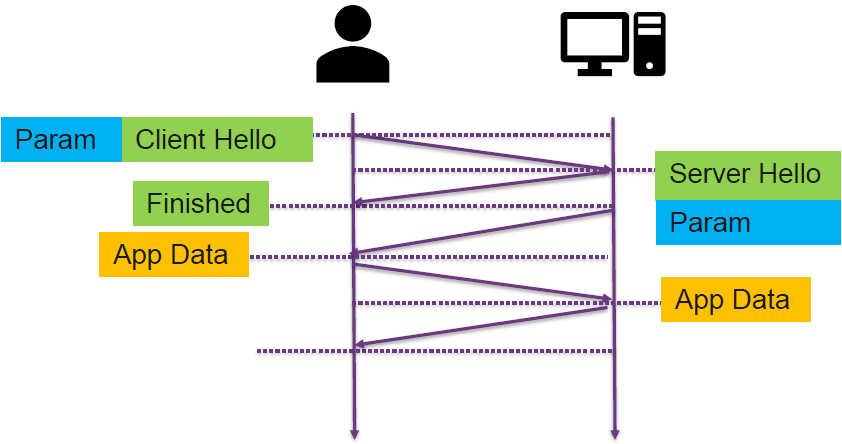
\includegraphics[width=0.8\linewidth]{img/quic.png}
\begin{itemize}
    \item Multiplexing in HTTP/2
    \item QUIC can multiplex requests: one stream does not affect others
\end{itemize}

\subsubsection{UDP}
\begin{itemize}
    \item Used for DNS, streaming
    \item Simple connectionless communication model
    \item No guarantee
    \begin{itemize}
        \item Delivery
        \item Ordering
        \item Duplicate protection
    \end{itemize}
\end{itemize}

\subsubsection{SCTP - Stream Control Transmission Protocol}
\begin{itemize}
    \item Message based
    \item Allows data to be divided into multiple streams
    \item Syn cookies: Four-way handshake with a signed cookie
    \item Multi-homing multiple IP addresses of endpoints
\end{itemize}